% Configuración a 2 columnas

%\documentclass[3p]{elsarticle}
\documentclass[3p,twocolumn]{elsarticle}

% Paquete con el tipo de codificación del lenguaje
\usepackage[utf8]{inputenc}
% Paquete para mostrar el número de líneas
\usepackage[modulo]{lineno}
\linenumbers
% Paquete para mostrar imágenes
\usepackage{graphicx}
\graphicspath{ {/home/acamon/TFG/GitHub/TFG/Recursos/Fotos/} }
% Paquete para resaltar enlaces y referencias
\usepackage{hyperref}
% Configuración del paquete
\hypersetup{
  breaklinks=true,  
  colorlinks=true,
  urlcolor=urlcolor,
  linkcolor=linkcolor,
  citecolor=citecolor,
}

% Modifica el formato de las referencias
\biboptions{sort&compress}

% Modifica el pie de la primera página para poner el número de la misma
\makeatletter
\def\ps@pprintTitle{%
   \let\@oddhead\@empty
   \let\@evenhead\@empty
   \def\@oddfoot{\reset@font\hfil\thepage\hfil}
   \let\@evenfoot\@oddfoot
}
\makeatother

% Paquete para cambiar color texto
\usepackage[dvipsnames]{xcolor}
% \textcolor{Red}{Hola}

% Paquete para las ecuaciones
\usepackage{amsmath}
\usepackage{lmodern}

% Paquete para escribir algoritmos y pseudocodigo
\usepackage[spanish,onelanguage,ruled,vlined]{algorithm2e} 

% Paquetes para la tabla
\usepackage{graphicx, caption}
\usepackage{booktabs}
\usepackage{threeparttable}


%====================================================================================================================================================%
%====================================================================================================================================================%


% Inicio del documento
\begin{document}

\title{TFG} % Título del TFG

\author[1]{Aarón Casado Monge} % Autor del TFG
\ead{aaron.casado@uah.es} % Correo del alumno

\author[2]{Juan José Cuadrado Gallego} % Tutor del TFG
\ead{jcg@uah.es} % Correo del profesor

% Dirección de la Escuela Politécnica Superior de UAH
\address{University of Alcala, Polytechnic School, Computer Science Department, Scientific and Technological Campus, Politechnic Building. Office: O243, 28805, Alcala de Henares, Madrid, Spain}

% Abstracto del TFG
\begin{abstract}
Clusterización (qué es y para qué sirve) - Técnicas (para qué sirven) - Paquetes 
\end{abstract}

% Palabras clave del TFG
\begin{keyword}
Data Mining, Clustering, R
\end{keyword}

\maketitle % Creación del Título, autores, abstracto...
 
 
%====================================================================================================================================================%
                                              %============================================================%
%====================================================================================================================================================%

 
% Introducción del TFG
\section{Introducción}

% Intento de poner una foto
%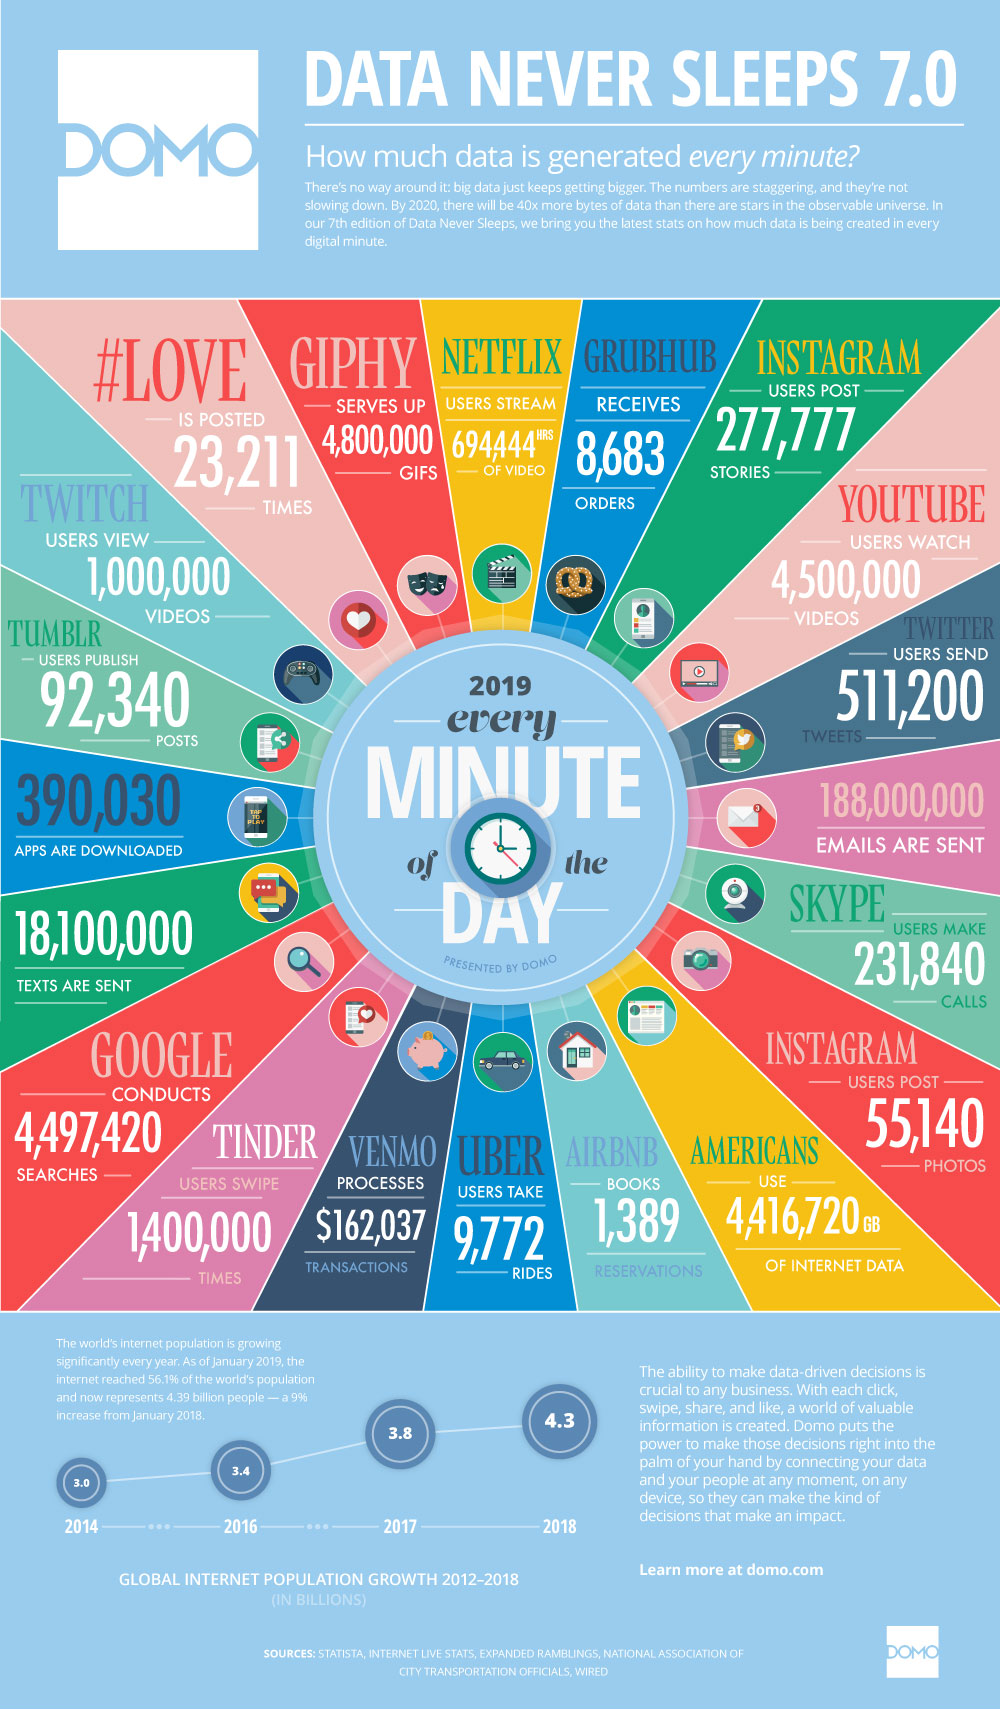
\includegraphics[width=\linewidth]{19_domo_data-never-sleeps-7}

Desde finales del sigo \textsc{xx} se ha considerado que vivimos en la ``era de la información'', una etapa caracterizada por el incremento, desarrollo y propagación de emergentes tecnologías de la información y comunicación que han permitido al ser humano romper las barreras de la distancia, el tiempo y el lugar a la hora de comunicarse y compartir información; actividades que han sido decisivas en nuestra historia \cite{1}. Sin embargo, la era en la que realmente vivimos es la ``era de los datos'', donde \textcolor{Red} {cada día se generan más de dos mil quinientos billones de petabytes\footnote {Un Petabyte es una unidad de información o almacienamiento de datos equivalente a un cuadrillon de bytes, mil terabytes o un millón de gigabytes. En este caso, es el equivalente a 2.5 quintillones de bytes.} de datos} provenientes de comercios, ciencias, Internet y casi cualquier actividad del día a día \cite{2} que acaban volcados en redes de ordenadores, sitios web, bases de datos y otros medios de almacenaje. 

Esta explosión de datos, a la que se ha denominado Big Data, se debe al alto grado de computarización de la sociedad y el avance de herramientas de recolección y almacenamiento de datos. Negocios en todo el mundo generan grandes cantidades de datos derivados de transacciones, stock de productos,  platillas de empleados, etc. Las ramas de la ciencia producen datos de manera constante frutos de experimentos, observaciones, recogida de muestras, etc. Y más recientemente, Internet y las redes sociales han sido las principales responsables del aumento excesivo de datos, siendo usadas por millones de personas simultáneamente.

Y, aunque esto ha supuesto una considerable mejora para la humanidad pues la información nunca había sido tan accesible, también ha traido consecuencias negativas y problemas como el almacenamiento y organización de los datos, datos no estructurados que entorpecen su acceso y procesamiento, dificultades a la hora de analizar los datos apropiadamente pudiendo generar desinformación y complicaciones para mostrar los resultados de forma apropiada y aplicarlos de manera eficiente y útil en el mundo real \cite{3}.

Como resultado, ha surgido una nueva ciencia que se ha posicionado rápidamente como una de las disciplinas más influyentes de la actualidad: Data Science (Ciencia de los Datos), que debido a su reciente aparición, carece de una definición consensuada, pero podríamos concretarla como ``\textit{Ciencia que usa Estadística, Inteligencia Artificial, Programación y Bases de Datos para posibilitar la extracción de conocimiento a partir de datos}'' \cite{4}. A su vez, dentro de esta ciencia se han desarrollado otras tres ramas: Data Warehousing, Data Mining y Visualization; cada una de ellas enfocada a resolver o afrontar uno o varios de los problemas mencionados previamente: organización y agrupación de datos, análisis de los mismos y presentación de los resultados, respectivamente.

De entre estas nuevas disciplinas, Data Mining es la que se centra en el procesamiento de los datos, procedimiento por el cual se obtiene la información, y se podría definir como ''\textit{Proceso de descubrimiento de patrones interesantes y conocimiento a partir de grandes volúmenes de datos}'' \cite{5}, donde dentro de la misma podemos encontrar diferentes técnicas para encontrar patrones y relaciones, y dependiendo de cuál se aplique se puede obtener un resultado totalmente diferente incluso con el mismo conjunto de datos, por lo que es fundamental emplear la técnica apropiada en función del del objetivo a conseguir, los datos con los que se pretende trabajar y el ámbito de aplicación.

Y en algunos de los campos más importantes del mundo moderno como la analítica de negocios, el reconocimiento de imágenes, las búsquedas web, seguridad, biología y ciencias de la salud; existen dificultades a la hora de clasificar o agrupar ciertos datos porque estos no disponen de una etiqueta o valor conocido por el que se pueda hacerlo, pues este no existe o no ha sido definido. Para poder afrontar este problema se utiliza la técnica de Clustering, que permite exactamente generar valores y etiquetas para un conjunto de datos realizando agrupaciones denominadas \textit{clusters} o grupos, donde los datos de un mismo cluster sean muy similares entre ellos y a su vez tengan diferencias claras con datos de otros clusters, permitiendo que cada grupo resultante puede ser etiquetado y tratado como una clase propia.

De esta manera, el objetivo de este Trabajo de Fin de Grado (TFG) es realizar un estudio sobre Clustering, exponiendo de manera teórica qué es este método y qué tipo de utilidades tiene, así como el desarrollo de las diferentes técnicas que existen y las aplicaciones que estas ofrecen. Posteriormente se explorará este método dentro de Bioinformática, un campo centrado en desarrollar técnicas y programas software para analizar datos biológicos, viendo qué aporta a dicha disciplina y cuáles de las técnicas expuestas previamente se emplean y por qué. 

Una vez realizado el marco teórico previo, se pretende hacer una parte práctica los diferentes paquetes que ofrecen técnicas de Clustering tanto de carácter general como dentro de Bioinformática para el lenguaje de programación R \cite{6}, uno de los más relevantes dentro de Data Science.


%====================================================================================================================================================%
                                              %============================================================%
%====================================================================================================================================================%


\section{Clustering} 

Clustering o Cluster Analysis, en español Agrupamiento o Análisis de Grupos y adaptado al término Clusterización, es un método de Data Mining que se basa en el Aprendizaje Automático (Machine Learning), una rama de la Inteligencia Artificial (Artificial Intelligence) que pretende desarrollar sistemas que resuelvan problemas basándose en los resultados de experiencias previas, aprendiendo de sus errores. Concretamente, se fundamenta en uno de los métodos de aprendizaje explorados en esta disciplina: Aprendizaje No Supervisado, enfocado en el desarrollo y descubrimiento de nuevos conocimientos. Este, a diferencia de otros métodos de aprendizaje, no dispone de conocimiento previo sobre lo que poder aprender, por lo que su objetivo principal es discernir patrones y relaciones entre los datos para poder separarlos \cite{7}.

En esencia, el proceso de Clustering es el mismo, hasta el punto en que básicamente podríamos considerarlos sinónimos, puesto que Clusterización se aplica principalmente sobre conjuntos de datos que se desean organizar en diferentes grupos pero los valores que delimitan cada cluster son desconocidos y por lo tanto se definen en el propio proceso de clasificación.

\textcolor{Red} {De una manera más técnica, podríamos decir que Clustering busca definir para una determinada característica\footnote{Dicho de una cualidad que da carácter o sirve para distinguir a algo o alguien de sus semejante.} o Suceso Elemental\footnote{Cada uno de los resultados más simples que se pueen obtener de la realización de un experimento. Obtener el número 3 al tirar un dado.} (SE), un conjunto de grupos de observaciones (suceso) \footnote{Se denomina así al subconjunto total de resultados posibles al realizar un experimento. Obtener un 3 o sacar par al tirar un dado.} con valores cercanos; donde los clusters permiten, dados los diferentes sucesos elementales que configuran un suceso, asignar cada SE al mismo cluster \cite{8}.}

Para poder decidir si dos datos deben ser agrupados en el mismo cluster o por el contrario, separados, es necesario introducir los conceptos de similaridad y disparidad; cuanto más similares sean los datos, más tendrán en común y por lo tanto es más probable que terminen bajo el mismo cluster, y por otra parte, si los datos son diferentes entre sí, serán separados en clusters diferentes. Este criterio se basa en la proximidad de dichos objetos. Si midiéramos la similitud entre dos objetos \textit{i} y \textit{j}, esta devolvería 0 si ambos fueran totalmente distintos, y cuanto más elevado fuera el valor, más semejantes serían, siendo 1 el valor más alto, indicando que ambos datos son idénticos. De la misma manera, medir la disparidad entre los objetos daría resultados opuestos, con un 0 indicando que son idénticos y con un 1 que no tienen nada en común. 

Esta forma de calcular la proximidad no solo ayuda a la hora de agrupar los datos en clusters y formar subconjuntos a partir de los resultados, sino que con este proceso también somos capaces de detectar outliers, datos anómalos que pueden ser datos erróneos procedentes de errores de medida o fallos que deben ser eliminados o, datos correctos sumamente importantes que son diferentes al esto y deben ser analizados detenidamente. A la hora de agrupar los datos, puede que queden varios objetos sueltos sin pertenecer a ningún cluster, esos son los datos anómalos.

Además, Clustering también sirve como primera aproximación a la hora de procesar los datos, porque aunque de por sí, este proceso puede aportar información útil agrupando datos similares y clasificándolos, permitiendo un análisis de los resultados que puede dar lugar al descubrimiento de nuevos conocimientos, también se usa como método de preprocesamiento de datos para otros algoritmos de Data Mining que trabajarán sobre las clusters generados y los atributos seleccionados como criterio a la hora de crearlos, pues estos se pueden considerar clases nuevas de objetos.

Es gracias a estas características que Clusterización es empleada en muchos ámbitos del mundo actual, siendo la técnica de Aprendizaje No Supervisado más extendida. Campos como la analítica de negocios, el reconocimiento de imágenes, las búsquedas web, seguridad, biología y ciencias de la salud hacen uso habitual de esta técnica para clasificar tipos de consumidores que comparten preferencias, aunar bajo un mismo subconjunto muchas formas diferentes de escribir el mismo caracter para facilitar el reconocimiento de textos escritos a mano, agrupar resultados similares de una consulta en internet y mostrar los más relevantes dentro de cada grupo o el estudio de la taxonomía\footnote{Ciencia que trata de los principios, métodos y fines de la clasificación. Se aplica en particular, dentro de la biología, para la ordenación jerarquizada y sistemática, con sus nombres, de los grupos de animales y de vegetales.} de las especies. También se puede hacer uso de su capacidad para detectar datos anómalos con la finalidad de revelar posibles fraudes o transacciones  financieras sospechosas, incluso ayudar en la disminución de crímenes analizando los resultados obtenidos tras clusterizar datos de detenciones y delitos; incluso aplicada a datos geofísicos\footnote{La Geofísica es la ciencia que estudia la Tierra desde el punto de vista de la física.} para interpretarlos y obtener resultados significativos. Asimismo, se utiliza a la hora de comparar comunidades en redes sociales permitiendo recomendar a los usuarios contenido de su agrado, o dentro del mundo sanitario, ayudando en la identificación y control de diversos tipos de enfermedades e incluso puede usarse como apoyo en la gestión de edificios públicos como bibliotecas, agrupando a los lectores por sus preferencias de manera similar a los consumidores de un negocio \cite{9,10,11,12,13}.

Comprimiendo toda esta información, podemos concretar los tres principales motivos por los que Clustering es empleado: clasificación natural tanto de individuos, como de objetos, etc.;, compresión de información para mayor facilidad a la hora de mostrar resultados y generación de una estructura base para el posterior tratamiento de los datos \cite{14}.

La utilidad de este método y la flexibilidad que ofrece con las diversas técnicas y formas de aplicarlo de las que dispone e es también parte fundamental de que sea tan comúnmente utilizado y con objetivos tan dispares en gran parte de las áreas del conocimiento. Sin embargo, también es un método frágil, pues depende en gran medida de los datos con los que se trabaje y el criterio escogido para determinar si dos objetos deben agruparse bajo el mismo cluster o separarlos, Por lo que es necesario seguir una serie de pasos a la hora de realizar un Análisis de Grupos de manera correcta \cite{15}:

\begin{enumerate}
  \item Primero, hay que seleccionar cuidadosamente los datos con los que se va a trabajar, puesto que tanto el tipo de dato como la cantidad de los mismos influyen directamente en los resultados. Si se utilizan demasiados datos el procesamiento puede tener un coste computacional alto y es difícil ofrecer una visualización elegante de los resultados. Pero si se escogen pocos datos se pierde información útil y puede dar lugar a equivocaciones. Es por ello que este paso suele realizarlo un experto en el sector o con su ayuda. 
  \item Segundo, se debe elegir la forma en la que se va a calcular la similaridad entre los diferentes datos, que analizaremos más adelante cuando analicemos las diferentes técnicas de Clustering.
  \item Tercero, debe definirse el criterio con el que se va a tomar la decisión de agrupar en el mismo cluster dos datos. Es decir, escoger el umbral de similaridad a partir del cual dos datos pasan a formar parte del mismo cluster y qué característica o conjunto de ellas van a ser utilizadas para medir la similitud. La elección del umbral suele ser complicada, y es necesaria mucha experiencia o varias iteraciones de ensayo y error para encontrar un valor correcto.
  \item Cuarto, hay que optar por uno de los diversos algoritmos de Clusterización que existen, pues los resultados pueden cambiar considerablemente al variar la estrategia con la que se realiza la agrupación. Estos se verán a continuación.
  \item Por último, una vez obtenidos los resultados hay que validarlos e interpretarlos. La resolución de este paso depende del objetivo inicial por el que se haya decidido realizar el análisis.
\end{enumerate}

Como puede verse, tanto el paso inicial como el último requieren de la ayuda de personas cualificadas si pretenden realizarse correctamente, y es en los pasos intermedios donde la intervención de computadoras y programas informáticos son más útiles y están más desarrollados, pues permiten aligerar considerablemente la carga de trabajo y como consecuencia, se puede analizar una mayor cantidad de datos. Pero no deja de ser una tarea complicada que ha ocasionado una gran demanda de expertos en Data Mining y Data Science en diversas áreas de trabajo durante los últimos años.

La utilidad que aporta Clustering permitiendo crear grupos con datos similares entre sí y dispares con respecto a otros grupos con el fin de clasificarlos y las ventajas que esto presenta queda reflejada en la cantidad de usos que recibe, por lo que vamos a profundizar en las diferentes técnicas que son empleadas para la generación de los clusters y su funcionamiento que lo hacen tan importante.


%====================================================================================================================================================%
                                              %============================================================%
%====================================================================================================================================================%

\section{Técnicas de Clustering} \label{sec:Técnicas de Clustering}

Existe una gran variedad de técnicas de Clustering que cumplen con el propósito de clasificar un conjunto de datos, pero no todas son iguales. Existen una serie de requisitos típicos que debe cumplir un algoritmo de Clusterización para satisfacer las expectativas y realizar un buen análisis. Sin embargo, cumplir todos estos requerimientos de forma simultánea es una tarea casi imposible, por lo que analizar cuáles ofrece cada algoritmo nos ayuda a identificar sus puntos fuertes y débiles y por ende, facilitar la elección del algoritmo apropiado para cada ocasión. Veamos cuáles son dichos requisitos y cómo podemos comparar algoritmos.

\subsection{\textbf{Requisitos de un algoritmo de Clustering}} \label{subsec:Requisitos de un algoritmo de Clustering}

\cite{16} Sobre el papel, analizar datos no debería suponer un problema; pero la realidad es que existen trabas que complican este procedimiento tales como la cantidad de datos a analizar o el tipo de datos. Algunos de los algoritmos de Clustering iniciales no tenían en cuenta este tipo de problemas, porque no existían en su momento, pero ahora es necesario afrontarlos para que el análisis de los datos sea eficiente y produzca resultados completos y veraces.

A continuación, se exponen los requisitos típicos que se exigen dentro de Data Mining a un algoritmo de Clustering, así como debilidades que presentan algunos de los existentes.

\begin{itemize}
  \item \textbf{Escalabilidad}: Muchos algoritmos de Clusterización trabajan bien con conjuntos de datos pequeños que contienen solo unos cuantos cientos de objetos; sin embargo, la gran mayoría de bases de datos contienen millones y miles de millones de datos. Analizar solo un pequeño porcentaje de esos datos puede resultar en conocimiento parcial, siendo necesario que sean escalables para resultados óptimos.
  
  \item \textbf{Habilidad para lidiar con diferentes tipos de atributos}\footnote{Dicho de una característica cualitativa de un individuo o dato usada para distinguirlo de una variable o característica cuantitativa.}: Coloquialmente se suele entiende por atributo un dato\footnote{Valor obtenido para una característica en una observación.} cuantitativo, es decir, un número. Sin embargo, existen otros tipos de datos: nominales\footnote{Dicho de un dato cualitativo que proporciona suficiente información para nombrar a una característica y poder diferenciarla de otra.}, binarios\footnote{Datos que solo pueden tomar los valores cero y uno (0, 1).}, ordinales\footnote{Datos cualitativos que proporcionan suficiente información para ordenar las observaciones.}, imágenes, gráficos, documentos y mezclas de varios de estos tipos. Por lo que un algoritmo de Clustering debe estar preparado para lidiar con todos o la gran mayoría de ellos.
  
  \item \textbf{Descubrimiento de clusters con formas arbitrarias}: Gran parte de los algoritmos utilizan formas de calcular la similaridad entre los datos basadas en la distancia entre los mismos, lo que suele dar lugar a clusters con formas redondas o esféricas. En determinadas ocasiones esto puede resultar contraproducente y erróneo, por lo que también es preciso que los algoritmos sean capaces de identificar diferentes formas de clusters, no solamente formas circulares o geométricas.
  
  \item \textbf{Requirir información al usuario}: En algunos algoritmos de Clustering es común pedir cierto tipo de información al usuario a la hora de trabajar con los datos, como el número de clusters que se quieren generar. Este tipo de práctica puede ocasionar problemas dada la complejidad de esta decisión, sobre todo en escenarios en los que los datos cuentan con múltiples atributos. Por lo que es recomendable que los algoritmos eviten este comportamiento tanto para aliviar a los usuarios como para no comprometer la calidad a la hora de formar clusters, pues el algoritmo se adaptaría al valor introducido por el usuario, aunque fuese erróneo, generando también, un resultado errado.
  
  \item \textbf{Capacidad para trabajar con ruido en los datos}: Aunque es común tratar de antemano los datos para eliminar cualquier tipo de dato no deseado, recordemos que esta técnica también se aplica como método de preprocesamiento para otros algoritmos de Data Mining, por lo que es necesario que no sean sensibles hacia estas impurezas, puesto que podría resultar en una clasificación pobre.
  
  \item \textbf{Clusterización incremental e insensibilidad al orden de entrada}: Cuando se aplica Clustering en entornos en constante movimiento como el de los negocios, es común que se introduzcan datos nuevos junto a los ya existentes. Ciertos algoritmos no son compatibles con este incremento de información, y es necesario volver a iniciar un nuevo proceso de Clusterización. Mientras que otros que sí toleran este cambio, resulta que son sensibles respecto al orden con el que se han introducido los datos y pueden generar agrupaciones erróneas. Estos problemas han dado lugar a la necesidad de algoritmos que puedan lidiar con la incorporación de nuevos datos y que no se vean afectados por el orden en el que estos son introducidos.
  
  \item \textbf{Capacidad de Clusterizar datos con muchos atributos}: Aunque de manera común se suele trabajar con datos que no contienen mucho más que una decena de atributos, hay ciertos tipos de datos como documentos, en los que cada palabra clave puede ser considerada un atributo, dando lugar a cientos de atributos por cada dato, haciendo complicado trabajar con ellos y también clasificarlos, por lo que se precisa de algoritmos que puedan lograr un buen resultado con este tipo de datos.
  
  \item \textbf{Clustering basado en restricciones}: En el mundo real podemos encontrar ciertas barreras a la hora de aplicar un algoritmo de Clustering, en los que, por ejemplo, sí se tenga que tener en cuenta un límite a la cantidad de cluster que se pueden generar o de decidir si dos datos o clusters deban unirse. Aunque es complicado realizar este tipo de agrupaciones, es indispensable que los algoritmos obtengan resultados decentes dadas estas limitaciones.
  
  \item \textbf{Interpretabilidad y usabilidad}: De nada sirve clasificar los datos y cumplir con los requisitos previos si no se puede interpretar el resultado. Los algoritmos, por lo tanto, deben ofrecer conclusiones comprensibles, coherentes y que puedan usarse, sometiéndose a ciertas limitaciones semánticas y visuales con la finalidad de acomodar el resultado al objetivo inicial por el que se ha llevado a cabo la clusterización.
\end{itemize}


%====================================================================================================================================================%


\subsection{\textbf{Criterios de comparación}} \label{subsec:Criterios de comparación}

\cite{16} Cada algoritmo opera de forma distinta en diferentes aspectos como el criterio de división, la separación de clusters, el cálculo de la similaridad y el espacio de clusterización. Observando los pasos a seguir y la toma de decisiones de un algoritmo, podemos compararlo con otro y escoger cuál es más adecuado para el problema a afrontar. 

\begin{itemize}
  \item \textbf{Criterio de división}: Principalmente existen dos tipos de métodos respecto a este criterio, aquellos que fraccionan todos los datos para que no exista ningún tipo de orden o diferencia de nivel entre ellos, y los que, por el lado opuesto, dividen los datos de manera jerárquica, permitiendo formar clusters en diferentes niveles semánticos. Cada uno aporta una utilidad distinta, con el primer tipo de criterio podemos abordar problemas como la clasificación de clientes o lectores, conjuntos de datos en los todos reciben el mismo trato; mientras que con criterio de partición jerárquico podemos organizar documentos en varios campos como ``deportes'', ``política'' o ``comida'', y dentro de cada campo tener subconjuntos como ``postres'', ``pasta'' o ``carne''.
  
  \item \textbf{Separación de clusters}: Otro criterio en el que hay dos enfoques: si un dato forma parte de un cluster, este no puede formar parte de otro a no ser que ambos clusters se unan; o permitir que un dato pueda estar en dos clusters a la vez, un concepto denominado ``Fuzzy clustering''. La primera aproximación ofrece un enfoque más determinista que es quizás el más aplicado entre ambos métodos, pero existen disciplinas en las que permitir que un dato forme parte de más de cluster puede ser realmente útil y que cada vez recibe más usos \cite{17}.  
  
  \item \textbf{Cálculo de similaridad}: Una de las pautas que más determina un algoritmo de clusterización es la forma en la que calculan la similaridad entre los datos, y que exploraremos detalladamente más adelante. Gran parte de los algoritmos utilizan la distancia que hay entre dos objetos para calcular su similaridad aplicando métodos como la distancia Euclídea o espacios vectoriales. Esta tipo de cálculo se ve beneficiado de métodos de optimización, pero suele generar clusters con formas esférica o cilíndricas, por lo que cada vez más se utilizan algoritmos que miden la similaridad entre objetos mediante la densidad o contigüidad del espacio para formar clusters, lo cual permite descubrir grupos con formas arbitrarias.  
  
  \item \textbf{Espacio de Clusterización}: Muchos algoritmos de Clustering observan todo el espacio de datos para buscar grupos, que es un método totalmente factible y válido para datos con pocos atributos. Sin embargo, cuando se tratan de procesar datos con gran cantidad de atributos, es mejor centrarse en pequeñas partes del total, en subconjuntos de espacio y buscar clusters dentro de ellos de forma que se pueda obtener información valiosa a un menor coste computacional.
\end{itemize}


%====================================================================================================================================================%


\subsection{\textbf{Clasificación general de técnicas}} \label{subsec:Clasificación general de técnicas}

\cite{16} Una vez que hemos visto los requisitos de los algoritmos de Clustering y los criterios para compararlos entre sí, podemos agrupar la mayor parte de las técnicas bajo cuatro grandes grupos basados principalmente en el cálculo de la similaridad y el criterio de división. Hablaremos brevemente sobre estos a continuación y posteriormente, precisaremos de manera individual sobre cada uno de ellos en las secciones \ref{sec:Métodos basados en particiones}, \ref{sec:Métodos jerárquicos}, \ref{sec:Métodos basados en densidad} y \ref{sec:Métodos basados en rejilla}, señalando los principales algoritmos dentro de cada una de ellos.

\begin{itemize}
  \item \textbf{Métodos basados en particiones}: Este tipo de métodos dividen todos los objetos de un conjunto de datos en clusters en los que debe haber al menos un objeto; o dicho de una forma más técnica, teniendo $n$ objetos, se generarán $k$ particiones siendo $k \leq n$. 
  
  Normalmente las técnicas de este grupo generan clusters exclusivos, donde un datos solo puede pertenecer a un cluster, pero cada vez se desarrollan más algoritmos de tipo fuzzy que relajan la agrupación. Asimismo, muchos de estos métodos calculan la distancia entre los objetos como medida de similaridad y generan de manera inicial $k$ particiones para posteriormente, de forma iterativa, tratar de reagrupar los datos y clusters para mejorar la clasificación, basándose en que los datos dentro del mismo cluster estén realmente cerca entre sí, y que con los datos de otros clusters se encuentren lejos. 
  
  Estos métodos sirven tanto para búsquedas en todo el espacio, como Clusterización de espacios reducidos, pero cuando la cantidad de atributos es muy alta, es preferible aplicarlos en subconjuntos, pues es complicado optimizar computacionalmente este tipo de algoritmos a la hora de generar las particiones iniciales, y para lidiar con este inconveniente, se suelen usar métodos heurísticos como \textit{$k$-means} que mejoran la calidad de Clustering progresivamente. Sin embargo, como se ha mencionado previamente, esta aproximación de Clustering genera grupos con formas esféricas y circulares, por lo que uno de los principales focos de mejora de estos algoritmos es evitar ese tipo de comportamiento cuando se trabaja con grandes conjuntos de datos.
  
  \item \textbf{Métodos jerárquicos}: Las técnicas de este grupo crean, como su propio nombre indica, una separación jerárquica de los datos. De forma diferente a los métodos basados en particiones donde todos los datos están en el mismo nivel, aquí se busca generar varios rangos para la Clusterización. 
  
  Existen dos enfoques principales dependiendo de cómo se generen los clusters: \textit{aglomerativo} y \textit{divisivo}. Las técnicas aglomerativas parten de la separación de todos los objetos en clusters individuales y progresivamente los va uniendo hasta que solo queda uno; mientras que las técnicas divisivas parten de un solo cluster inicial en el que se encuentran todos los objetos y va formando clusters más pequeños hasta que cada objeto es en sí un cluster. Es por eso que también se les conoce por métodos de ``abajo a arriba'' y de ``arriba a abajo'' respectivamente.
  
  Esta técnicas pueden utilizar distancia, densidad y continuidad como medida de calcular la similaridad entre los datos y son útiles tanto en búsquedas de espacios completos como de subconjuntos.
  
  \item \textbf{Métodos basados en densidad}: Este tipo de métodos surgieron como solución a los métodos basados en particiones y su tendencia a encontrar únicamente clusters con formas esféricas o circulares, puesto que las técnicas que utilizan la densidad del espacio a la hora de formar clusters permiten descubrir clusters con formas más arbitrarias. 
  
  El concepto general de estos métodos consiste en agrandar un cluster mientras la densidad en el ``vecindario'' este por encima de un umbral. La densidad se calcula por la cantidad de objetos que hay en el espacio de datos y el vecindario hace referencia a todos los datos que se encuentran a cierta distancia de un objeto determinado.
  
  El concepto general es que para cada objeto dentro de un cluster, en su vecindario de radio $r$ de distancia debe haber un mínimo de $x$ objetos. Este tipo de aproximación resulta muy conveniente a la hora de detectar datos anómalos.
  
  Los métodos basados en densidad pueden clasificar los datos en clusters exclusivos o de manera jerárquica, y aunque normalmente consideran que un objeto solo puede pertenecer a un cluster, también existen técnicas fuzzy Clustering. Asimismo, se pueden aplicar tanto en espacios completos como en regiones puntuales.
  
  \item \textbf{Métodos basados en cuadrícula o rejilla}: Estos métodos dividen el espacio de objetos en una cantidad determinada de celdas que forman una estructura de cuadrícula o rejilla, de ahí su nombre. Todas las operaciones con los datos se realizan dentro de la rejilla, que permite un procesamiento mucho más rápido, pues no depende de la cantidad de datos, sino de la de celdas existentes.
  
  Esto permite que puedan ser integrados con otros métodos de clustering de otros grupos como jerárquicos y basados en densidad para mejorar su eficiencia.
\end{itemize}

En la tabla \ref{Tab:Tabla 1} se han resumido estos grupos y las principales características de los mismos. Cabe mencionar que esta clasificación no es perfecta, pues existen algoritmos que integran conceptos de diferentes métodos. 

A continuación, exploraremos todos estos grupos y las principales técnicas empleadas en cada uno de ellos.


\begin{table*}[ht]
  \centering
  \caption{Resumen de métodos de Clusterización}
  \label{Tab:Tabla 1}
  \resizebox{\linewidth}{!}{%
  \begin{tabular}{|l|l|}
    \hline
    \textbf{Método} & \textbf{Características generales} \\ \hline
    \begin{tabular}[c]{@{}l@{}}Basados en \\ particiones\end{tabular} & \begin{tabular}[c]{@{}l@{}}- Encuentran clusters de forma esférica mutuamente exclusivos\\ - Utilizan distancia/proximidad\\ - Usan la media o medoid para representar el centro del cluster\\ - Efectivos en conjuntos de datos pequeños y medianos\end{tabular} \\ \hline
    Jerárquicos & \begin{tabular}[c]{@{}l@{}}- Clasifican en múltiples niveles\\ - No pueden deshacer agrupaciones o divisiones erróneas\\ - Pueden incorporar otras técnicas como microclustering y tener en cuenta vínculos entre los objetos\end{tabular} \\ \hline
    \begin{tabular}[c]{@{}l@{}}Basados en \\ densidad\end{tabular} & \begin{tabular}[c]{@{}l@{}}- Pueden encontrar clusters con formas arbitrarias\\ - Los clusters son regiones con gran densidad de objetos separados por zonas con poca densidad\\ - La densidad queda definida por un mínimo de objetos cercanos dentro del vecindario\\ - Sirve para detectar datos anómalos\end{tabular} \\ \hline
    \begin{tabular}[c]{@{}l@{}}Basados \\ en rejilla\end{tabular} & \begin{tabular}[c]{@{}l@{}}- Utiliza una estructura de rejilla o cuadrícula\\ - La velocidad de procesamiento es alta, pues no influye el número de objetos\end{tabular} \\ \hline
    \end{tabular}%
  }
\end{table*}


%====================================================================================================================================================%
                                              %============================================================%
%====================================================================================================================================================%


\section{Métodos basados en particiones} \label{sec:Métodos basados en particiones}

Los métodos pertenecientes a este grupo son quizás los más simples y básicos de Clustering. Estos organizan los datos de un conjunto en diversos clusters exclusivos, y es común que soliciten al usuario el número de grupos o clusters finales que debe haber, pues sirve como punto de partida para estos métodos. Esto permite simplificar su funcionamiento, pero a su vez, supone el incumplimiento de uno de los requisitos de los que se ha hablado previamente en la sección \ref{subsec:Requisitos de un algoritmo de Clustering}.

De forma técnica, dado un conjunto de datos $D$ con $n$ objetos y siendo $k$ el número de clusters a formar, un algoritmo basado en particiones organizará los objetos en $k$ divisiones, con $k \leq n$, donde cada una de ellas representa un cluster. 

Los clusters son generados intentando optimizar el criterio de similaridad, siendo uno de los más utilizados el del cálculo de proximidad, donde se intentan agrupar bajo el mismo clusters aquellos objetos que estén cerca en el espacio de datos y que a su vez, hacen que todos los datos de un cluster estén alejados de los objetos de otro cluster, asegurando de esta manera un alto grado de semejanza entre los del mismo cluster y diferencia con los de otros clusters.

A continuación se exponen los dos algoritmos más utilizados de este grupo y de los más conocidos: $k$-media ($k$-means) y $k$-medoids.


%====================================================================================================================================================%


\subsection{\textbf{\textit{k}-Means}} \label{subsec:k-means}

El objetivo de los algoritmos basados en particiones es, dado un conjunto de datos $D$ con $n$ objetos en un espacio Euclídeo\footnote{Espacio geométrico donde se satisfacen los axiomas de Euclides.}, formar $k$ clusters, $C_{1}, ..., C_{k}$, donde cada cluster es un subconjunto del conjunto de datos $C_{i} \subset D$ y la intersección entre clusters es nula $C_{i} \cap C_{j} = \emptyset$ para $i \leq j$ y $j \leq k$. Sin embargo, estos requieren de una gran capacidad computacional, y es por ello que algoritmos como $k$-Means son tan utilizados.

$k$-Means representa cada cluster con su ``centroide'', que es básicamente el punto central del cluster, y se calcula como la media de los puntos que lo forman. Para un conjunto de datos con dos atributos cuantitativos, la fórmula para calcular el centroide $c_{i}$ es la siguiente: \begin{equation} c_{i} = \left( \frac{\sum _{i=1}^n x_{i}}{n}; \frac{\sum _{j=1}^m y_{j}}{m} \right). \end{equation} 

Asimismo, otro de los métodos más comunes para medir la distancia entre puntos y clusters, y que también utiliza $k$-Means, es la distancia Euclídea. La fórmula de la distancia Euclídea entre dos puntos cualesquiera $dist(p, q)$ de un espacio Euclídeo $p$ y $q$, con coordenadas cartesianas\footnote{Tipo de coordenadas ortogonales usadas en espacios Euclídeos que tienen como referencia los ejes ortogonales.} $(x_{1}, y_{1})$ y $(x_{2}, y_{2})$ es como sigue: \begin{equation}  dist\left( p,q\right) =  \sqrt{ \left(x_1-x_2 \right)^2 + \left(y_1 - y_2 \right)^2}. \end{equation} 

Y para comprobar la calidad de un cluster, y garantizar que los objetos del un mismo sean similares entre ellos, pero diferentes con objetos de otros clusters, los métodos basados en particiones suelen utilizar la \textit{varianza} dentro del cluster, que es la suma del error cuadrático\footnote{Técnica para calcular la diferencia entre el estimador y lo que se estima.} entre todos los objetos del cluster $C_i$ y el centroide $c_i$, definida como: \begin{equation} E =  \sum_{i=1}^{k}  \sum_{p \in C_i} dist(p, c_i)^2 , \end{equation} donde $E$ es la suma del error cuadrático de todos los objetos pertenecientes al cluster $p_i \in C_i$. La finalidad de esta operación es asegurar que los $k$ cluster resultantes sean lo más compactos y distantes posible.

\textcolor{Red}{Es aquí, en el cálculo de la varianza donde la optimización de este método se vuelve computacionalmente complicada, pues en el peor de los casos, el total de posibles clasificaciones depende del número total de clusters de manera exponencial y posteriormente habría que comprobar los valores de la varianza dentro de cada cluster, siendo un problema de complexión NP-complejo\footnote{No se definir esto bien}.} Para resolverlo, se utilizan algoritmos voraces\footnote{Estrategia de búsqueda en la que se sigue una heurística que consiste en escoger la opción más optima en cada paso de manera local, esperando llegar a una solución general óptima.} como $k$-Means, que es simple y usado habitualmente.

Este algoritmo sigue una serie de pasos para formar los clusters y evaluar su calidad. Primero, selecciona $n$ objetos dentro del conjunto de datos $D$ para representar los clusters iniciales; y puesto que son los únicos integrantes de ellos, el cálculo del centroide da como resultado el propio objeto. Posteriormente, asigna cada uno de los objetos restantes al cluster con el que es más similar basándose en el cálculo de la distancia Euclidiana entre el objeto y representante del cluster. A partir de aquí, el algoritmo intenta mejorar los resultados de la varianza, para ello, vuelve a calcular el centroide de cada cluster con los nuevos objetos añadidos en la iteración previa, y reagrupa los objetos ahora con los representantes de cada cluster actualizados. El proceso continua hasta que los centroides, y por ende, clusters de la iteración actual sean idénticos a los de la iteración previa.

El pseudocódigo de $k$-Means queda resumido en el algoritmo \ref{alg:Algoritmo k-means}. 

\begin{algorithm}[ht]
\SetAlgoLined
  \LinesNumbered
  \SetKwRepeat{Do}{repetir}{hasta}
  \DontPrintSemicolon
  \KwIn{$k$: número de clusters, \\ $D$: conjunto de datos con $n$ objetos.}
  \KwOut{Un conjunto de $k$ clusters.}
  \Begin{
    selección arbitraria de $k$ objetos de $D$ como representantes de los clusters iniciales\;
    \Do{no hay cambios}{
      calcular la distancia de cada objeto al centroide de cada cluster\;
      (re)asignar cada objeto al cluster con el que es más similar en función de la distancia obtenida\;
      actualizar los centroides de los clusters con los nuevos objetos añadidos\;
    }
  }
  \caption{$k$-Means, basado en la media}
  \label{alg:Algoritmo k-means}
\end{algorithm}

Sin embargo, este método no garantiza converger hacia un máximo global, sino que muchas veces termina en un máximo local. El resultado depende de la selección de clusters iniciales sobre los que se trabaja, por lo que es es común realizar varias pruebas del algoritmo con diferentes clusters iniciales hasta encontrar un resultado óptimo. 

Por otro lado, la complejidad temporal de $k$-means es considerablemente baja  $O(nkt)$, pues depende del número de objetos $n$, del de clusters $k$ y de la cantidad de iteraciones $t$ y normalmente encontramos que $k \ll n$ y $t \ll n$. Lo cual sugiere que escalar este algoritmo a grandes conjuntos de datos es asequible.

Asimismo, este algoritmo solo puede ser utilizado cuando podemos calcular la media de varios objetos para encontrar el centroide, por lo que en casos donde los datos tengan atributos nominales, no se puede aplicar. Pero existen modificaciones y versiones de $k$-means que solucionan algunos de estos problemas, como $k$-modas, que en vez d utilizar la media para calcular el centroide, utiliza la moda, el atributo que más se repite para una característica, y si permite trabajar con datos nominales.

Otra de las desventajas que presenta y que comentábamos al inicio de la sección, es el hecho de que no cumple uno de los requisitos de los métodos de clustering, y es que $k$-means pide al usuario el número $k$ de clusters a generar como dato de entrada indispensable. Si bien es cierto que se han propuesto estudios para solventar este problema intentando encontrar el mejor valor para $k$ ejecutando varias veces el algoritmo con distintas unidades, pero supone un alto coste computacional. 

Además, recordemos que este algoritmo flaquea a la hora de encontrar clusters con formas poco convencionales y de tamaños dispares, siendo realmente sensible a datos anómalos e impurezas, que pueden alterar los cálculos de los centroides.


%====================================================================================================================================================%


\subsection{\textbf{\textit{k}-Medoids}} \label{subsec:k-Medoids}

Como se ha mencionado en el apartado previo \ref{subsec:k-means}, $k$-means es realmente susceptible a datos anómalos e impurezas, pues como estos objetos se suelen encontrar alejados de todos los datos, cuando se asignan a un cluster y se recalcula el valor del centroide, este valor se ve altamente alterado, lo cual tambíen afecta a la formación del resto de clusters.

Con el objetivo de ser menos sensible con estos datos, $k$-medoids utiliza uno de los objetos del cluster en vez de su centroide como representante del mismo, y el resto de objetos se añaden al cluster cuyo objeto representativo sea más similar. Por lo que el método para comprobar la calidad del cluster ya no es la varianza, sino el error absoluto, cuya fórmula es la siguiente: \begin{equation} \label{eq:k-medoids} E =  \sum_{i=1}^{k}  \sum_{ \in C_i} dist(p, o_i)^2 , \end{equation}, siendo $E$ la suma del error absoluto para todos los puntos $p_i$ pertenecientes al cluster $C_i$ $\left(p_i \in C_i \right)$ con respecto al objeto representativo de dicho cluster $o_i$. De esta manera, $k$-medoids agrupa $n$ objetos en $k$ clusters minimizando el error absoluto.

Los algoritmos más conocidos que utilizan esta aproximación para formar clusters son Partioning Around Medoids(PAM) y Clustering LARge Applications (CLARA), cada uno con sus propias características, que veremos a continuación.

%====================================================================================================================================================%

\subsubsection{\textbf{PAM}}

Este algoritmo, que podría traducirse al español como Particionamiento Sobre Medoids, es una de las aplicaciones más extendidas del método $k$-medoids, y tiene un funcionamiento similar a $k$-means en el sentido de que utiliza también una heurística voraz de forma iterativa para la formación de clusters y disminuir la complejidad computacional. 

Y de la misma forma, el paso inicial también es seleccionar de manera aleatoria $k$ objetos para formar los clusters iniciales, denominados ``semillas'', y asignar los objetos restantes al cluster cuyo objeto representativo (medoid) es el más similar. Posteriormente, con los nuevos clusters, se comprueba si cambiando el objeto representativo del cluster actual $o_i$ por otro objeto cualquiera dentro del cluster $o_{cualquiera}$ se mejora la calidad del cluster, y en caso de que sea así, se intercambia uno con otro. Esta comprobación se realiza para todos los objetos dentro del cluster que no son el representativo $o_{cualquiera} \neq o_i$ y para todos los clusters, hasta que no se puede mejorar la situación actual. Una vez ha terminado este proceso, se vuelve a calcular la similaridad entre todos los objetos y los representantes de los clusters y se reagrupan si es necesario. El algoritmo termina cuando los clusters resultantes de la iteración actual son idénticos a los de la previa. 

Para determinar la calidad del cluster y decidir si un representante de un cluster debe ser cambiado por otro se calcula la distancia entre todos los puntos de un cluster y su objeto representante actual $o_i$ mediante la fórmula \ref{eq:k-medoids}, cuyo resultado es almacenado. Luego, de forma iterativa cada objeto perteneciente al cluster se convierte en su representante $o_j$ temporal y se vuelve a calcular la distancia entre el resto de puntos y el representante temporal, y su resultado también se almacena, de forma que, una vez todos los puntos han sido representantes, se escoge como representante aquel cuyo resultado ha sido el más bajo, es decir, el más cercano a la mayoría de puntos del cluster, y si este nuevo punto es distinto al representante actual $o_i \neq o_j$, $o_j$ se convierte en el nuevo representante del cluster. 

Cuando un intercambio de representante ocurre en un cluster, se debe comprobar si es necesario reestructurar los clusters y el coste que esto conlleva, pues puede haber puntos cuyo cluster más cercano haya variado. Por lo que para cada punto del espacio de objetos se calcula la distancia a los nuevos representantes y se selecciona el que esté más cerca, pudiendo ser un nuevo cluster o el mismo en el que se encontraba pero con el nuevo representante. Una vez seleccionado el cluster más cercano para cada objeto, se calcula el coste con la misma función \ref{eq:k-medoids}, y si el resultado de esta reestructuración es negativo, es decir, si en la nueva situación los clusters representan mejor a los objetos porque el representante está más cerca de los puntos, se acepta este cambio y se considera que ha aumentado la calidad de los clusters.

\begin{algorithm}[ht]
\SetAlgoLined
  \LinesNumbered
  \SetKwRepeat{Do}{repetir}{hasta}
  \DontPrintSemicolon
  \KwIn{$k$: número de clusters, \\ $D$: conjunto de datos con $n$ objetos.}
  \KwOut{Un conjunto de $k$ clusters.}
  \Begin{
    selección arbitraria de $k$ objetos de $D$ como representantes $o_i$ de los clusters iniciales\;
    \Do{no hay cambios}{
      calcular la distancia de cada objeto al representante de cada cluster\;
      (re)asignar cada objeto al cluster con el que es más similar en función de la distancia obtenida\;
      seleccionar un objeto cualquiera del cluster que no sea el represente actual $o_{cualquiera}$\;
      calcular el coste $T$ de intercambiar el representante del cluster $o_i$ con $o_{cualquiera}$\;
      
      \If{T$<$0}{ intercambiar $o_i$ con $o_{cualquiera}$ como representante del cluster}´
    }
  }
  \caption{PAM, basado en representantes}
  \label{alg:Algoritmo PAM}
\end{algorithm}

Este procedimiento, que queda resumido en el algoritmo de PAM \ref{alg:Algoritmo PAM}, es más robusto que $k$-means al ser más tolerante a datos anómalos e impurezas, porque el medoid está menos influenciado por estos que la media. Sin embargo, esta aproximación es mucho más compleja computacionalmente para cada iteración y sigue solicitando el número de clusters $k$, por lo que para gŕandes volúmenes de datos resulta ineficiente, dando origen a otra versión enfocada precisamente a este tipo de trabajo: CLARA.


%====================================================================================================================================================%


\subsubsection{\textbf{CLARA}}

CLARA es una variación de PAM y que también aplica $k$-medoids a la hora de formar clusters, pero que en lugar de tener en cuenta todos los datos $n$ del conjunto de datos $D$, este algoritmo escoge una muestra aleatoria $m$ de datos y posteriormente aplica PAM para calcular los mejores representantes de la muestra, que idealemente, representa de una manera precisa a $D$ siempre y cuando cada objeto $p_i$ tenga las mismas posibilidades de ser escogido para la muestra. De esta manera y tras varias iteraciones seleccionando muestras arbitrarias, CLARA devuelve la mejor clusterización obtenida de todas ellas.

Esto permite que la complejidad computacional disminuya, pues la comprobación de la calidad de los clusters y el intercambio de representantes que tanto costaba en PAM es reducido de manera drástica con este enfoque, permitiendo de esta manera que pueda trabajar con grándes volúmenes de datos.

Sin embargo, este algoritmo depende totalmente de las muestras escogidas y la probabilidad de que el mejor representante de cada cluster se encuentre en ella, puesto que si tan solo uno de ellos no aparece en alguna de las muestras, CLARA nunca encontrará la mejor clusterización posible. 


%====================================================================================================================================================%
                                              %============================================================%
%====================================================================================================================================================%


\section{Métodos jerárquicos} \label{sec:Métodos jerárquicos}

Mientras que los métodos basados en particiones cumplen con el requisito básico de agrupar los datos en clusters exclusivos, hay ocasiones en las que clasificar los datos en diferentes niveles, es decir, de forma jerárquica, puede proporcionar grandes ventajas. De esta manera, los métodos jerárquicos organizan los datos en una jerarquía o árbol de clusters. 

Útil en escenarios donde los datos tengan de por sí cierta estructura jerárquica (estructura de empleados) o en aquellos en los que se pretenda descrubir si existe una oculta(teroría de la evolución), estos métodos se clasifican a su vez en dos grupos: aglomerativos y divisivos. 

\begin{itemize}
  \item \textbf{Métodos jerárquicos aglomerativos}: Estos métodos utilizan una estrategia de ``abajo a arriba'', partiendo de que cada objeto compone su propio cluster y de forma iterativa los va uniendo en clusters más grandes hasta que solo queda un único cluster, que se conoce como ``raiz''. En cada iteración se mergen los dos clusters más cercanos entre sí para formar uno solo.

  \item \textbf{Métodos jerárquicos divisivos}: Este tipo de métodos utilizan una estrategia de ``arriba a abajo'', donde situa a todos los objetos en un cluster inicial, la raiz, y de manera progresiva divide la raiz en subclusters más pequeños sucesivamente hasta que cada cluster queda formado únicamente por un objeto o los objetos de cada cluster son prácticamente idénticos entre sí.
\end{itemize}

Como se puede ver, son métodos opuestos pero que operan bajo el mismo principio. Sin embargo, es mucho más complicado dividir los datos que juntarlos, pues hay muchas más posibilidades y por lo tanto más comprobaciones que realizar; dando lugar a que los métodos aglomerativos sean más comunes y los divisivos dependan de métodos heurísticos que pueden dar resultados inexáctos.

Los métodos jerarquicos pueden sufrir dificultades a la hora de dividir o juntar clusters, una parte crítica en su procedimiento, puesto que, a diferencia de los métodos basados en particiones donde en cada iteración se reagrupaban los puntos hacia el cluster más cercano, si un método jerárquico divide o junta dos clusters, no hay vuelta atrás y los siguiente pasos trabajarán con el resultado obtenido sin poder cambiarlo. Por lo que decidir cómo y por qué motivo se genera un cluster es una tarea complicada, que de no ser correcta, puede ocasionar resultados pobres. Y la otra desventaja principal de este enfoque es que no escalan bien hacia grandes volúmenes de datos, puesto que deben realizar muchas comprobaciones cuando se queieren unir o separar clusters.

Para lidiar con estos problemas se han desarrollado técnicas como BIRCH y Chameleon de las que se habla en la \textcolor{Red}{sección X}, que incorporan métodos jerárquicos con otros métodos, resultando en otros tipos de clustering conocidos como multi fase y microclustering.

Antes de explicar algunos de los algoritmos más utilizados dentro de este grupo, analicemos brevemente las diferentes maneras que existen en los métodos jerárquicos para medir distancias.


%====================================================================================================================================================%


\subsection{Medidas de distancia} \label{Medidas de distancia}

Independiéntemente del tipo de método que se utilice, aglomerativo o divisivo, se necesita una forma de medir la distancia entre dos clusters, puesto que aquí no se escoge un representante del cluster para realizar este tipo de cálculos. 

Existen tres formas diferentes de realizar este cálculo. \\

\begin{itemize}
  \item \textbf{Distancia mínima}: Esta define la proximidad entre dos clusters como la distancia entre los puntos más cercanos entre ambos, también conocida como ``single link''.
\begin{equation} dist_{min}(C_i, C_j) =  \min_{p \in C_i, p' \in C_j} \left\{|p - p'|\right\} \end{equation}

  \item \textbf{Distancia maxima}: Define la proximidad entre dos clusters como la distancia entre los puntos más alejados entre ellos, también conodida como ``complete link''.
\begin{equation} dist_{max}(C_i, C_j) =  \max_{p \in C_i, p' \in C_j} \left\{|p - p'|\right\} \end{equation}

\textbf{Distancia media}: Define la proximidad entre dos clusters como la distancia media entre todos los puntos de ambos clusters.
\begin{equation} dist_{avg}(C_i, C_j) = \frac{1}{n_i \cdot n_j} \sum_{p \in C_i, p' \in C_j} |p - p'|  \end{equation}
\end{itemize}

Las dos primeras son medidas que se van a los extremos y son susceptibles a datos anómalos e impurezas, por lo que el uso de la media es un compromiso entre ambas para solventar este problema.


%====================================================================================================================================================%


\subsection{AGNES} \label{subsec:AGNES}


%====================================================================================================================================================%


\subsection{DIANA} \label{subsec:DIANA}


%====================================================================================================================================================%


\subsection{BIRCH} \label{subsec:BIRCH}


%====================================================================================================================================================%


\subsection{Chameleon} \label{subsec:Chameleon}


%====================================================================================================================================================%


\subsection{Métodos jerárquicos probabilísticos} \label{subsec:Métodos jerárquicos probabilísticos}


%====================================================================================================================================================%
                                              %============================================================%
%====================================================================================================================================================%

\clearpage

\section{Métodos basados en densidad} \label{sec:Métodos basados en densidad}


%====================================================================================================================================================%
                                              %============================================================%
%====================================================================================================================================================%


\section{Métodos basados en rejilla} \label{sec:Métodos basados en rejilla}



%====================================================================================================================================================%
                                              %============================================================%
%====================================================================================================================================================%
%====================================================================================================================================================%
                                              %============================================================%
%====================================================================================================================================================%
%====================================================================================================================================================%
                                              %============================================================%
%====================================================================================================================================================%
%====================================================================================================================================================%
                                              %============================================================%
%====================================================================================================================================================%
%====================================================================================================================================================%
                                              %============================================================%
%====================================================================================================================================================%%====================================================================================================================================================%
                                              %============================================================%
%====================================================================================================================================================%%====================================================================================================================================================%
                                              %============================================================%
%====================================================================================================================================================%
%====================================================================================================================================================%
                                              %============================================================%
%====================================================================================================================================================%
%====================================================================================================================================================%
                                              %============================================================%
%====================================================================================================================================================%

\clearpage

\renewcommand{\contentsname}{\section{Índice}}
\tableofcontents

\renewcommand{\listalgorithmcfname}{\section{Algoritmos}}
\listofalgorithms

\renewcommand{\listtablename}{\section{Tablas}}
\listoftables

\renewcommand{\listfigurename}{\section{Imágenes y figuras}}
\listoffigures

\section{Referencias}
\renewcommand{\section}[2]{}
\begin{thebibliography}{X}

\bibitem{1} Alberts, D. S., \& Papp, D. S. (1997). \href{http://www.dodccrp.org/files/Alberts_Anthology_I.pdf} {The information age: An anthology on its impact and consequences}. Office of the Assistant Secretary of Defense Washington DC Command and Control Research Program (CCRP).

\bibitem{2} Becoming A Data-Driven CEO | Domo. (2018). Data never sleeps 6.0 \href{https://www.domo.com/solution/data-never-sleeps-6} {https://www.domo.com/solution/data-never-sleeps-6}

\bibitem{3} Xu, Z., \& Shi, Y. (2015). \href {https://link.springer.com/content/pdf/10.1007/s40745-015-0063-7.pdf} {Exploring big data analysis: fundamental scientific problems}´. Annals of Data Science, 2(4), 363-372.

\bibitem{4} Definición Data Science apuntes FCD

\bibitem{5} Definición Data Mining libro 100

\bibitem{6} The R Project for Statistical Computing. (n.d.). Retrieved from \href{https://www.r-project.org/} {https://www.r-project.org/}

\bibitem{7} Moreno, A. (1994). \href{https://upcommons.upc.edu/bitstream/handle/2099.3/36157/9788483019962.pdf?sequence=1&isAllowed=y} {Aprendizaje automático.} Llibre, Edicions UPC.

\bibitem{8} Apuntes JJ clustering

\bibitem{9} Alkhaibari, A. A., \& Chung, P. (2017). \href{https://ieeexplore.ieee.org/document/8001983} {Cluster analysis for reducing city crime rates}. 2017 IEEE Long Island Systems, Applications and Technology Conference (LISAT). doi:10.1109/lisat.2017.8001983

\bibitem{10} Song, Y., Meng, H., \& Zhang, Y. (2010). \href{https://ieeexplore.ieee.org/document/5602787} {Clustering analysis and its applications}. 2010 Second IITA International Conference on Geoscience and Remote Sensing. doi:10.1109/iita-grs.2010.5602787

\bibitem{11} Prabhu, J., Sudharshan, M., Saravanan, M., \& Prasad, G. (2010). \href{https://ieeexplore.ieee.org/document/5563072} {Augmenting Rapid Clustering Method for Social Network Analysis}. 2010 International Conference on Advances in Social Networks Analysis and Mining. doi:10.1109/asonam.2010.55

\bibitem{12} Baron, J. N., Aznar, M. N., Monterubbianesi, M., \& Martínez-López, B. (2020). \href{https://search.ebscohost.com/login.aspx?direct=true&db=aph&AN=143827917&lang=es&site=ehost-live&scope=site} {Application of network analysis and cluster analysis for better prevention and control of swine diseases in Argentina}. PLoS ONE, 15(6), 1–26. https://doi.org/10.1371/journal.pone.0234489

\bibitem{13} Li, J., \& Chen, P. (2008). \href{https://ieeexplore.ieee.org/document/4810639} {The application of Cluster analysis in Library system}. 2008 IEEE International Symposium on Knowledge Acquisition and Modeling Workshop. doi:10.1109/kamw.2008.4810639

\bibitem{14} Emebo, O., Aromolaran, O., Oyelade, J., Isewon, I., Oladipupo, O., Omogbadegun, Z., ... Olawole, O. (2019). Data Clustering: Algorithms and Its Applications. 2019 19th International Conference on Computational Science and Its Applications (ICCSA). doi:10.1109/iccsa.2019.000-1

\bibitem{15} Carugo, O., \& Eisenhaber, F. (2010). Data Mining Techniques for the Life Sciences. Humana Press.
             
\bibitem{16}Han, J., Kamber, M., \& Pei, J. (2012). Data Mining: Concepts and Techniques (3rd ed., p.~740). 225 Wyman Street, Waltham, MA 02451, USA: Morgan Kaufmann Publishers, Elsevier.

\bibitem{17} Höppner, F., Klawonn, F., Kruse, R., \& Runkler, T. (1999). Fuzzy cluster analysis: methods for classification, data analysis and image recognition. John Wiley \& Sons.


\end{thebibliography}

\end{document}